\section[Rappels]{Rappels}

\subsection{Probabilité conditionnelle}

\begin{frame}{Probabilité conditionnelle}
	Le théorème de Bayes découle naturellement de la définition d'une probabilité conditionnelle:
	\begin{block}{Définition: probabilité conditionnelle}
		\'Etant donné deux événements $A$ et $B$, on définit la probabilité conditionnelle de $A \mid B$, qui se lit \textit{A sachant B}, comme le rapport entre la probabilité jointe de $A$ \textbf{et} $B$ et la probabilité marginale de $B$:
		\begin{equation}
			P(A \mid B) = \displaystyle \frac{P(A \cap B)}{P(B)}
			\nonumber
		\end{equation}
	\end{block}
\end{frame}

\begin{frame}{Probabilité conditionnelle}
	Lorsque les événements $A$ et $B$ sont indépendants, on peut écrire:
	\begin{equation}
		P(A \cap B) = P(A) \, P(B)
		\nonumber
	\end{equation}
	\pause
	La probabilité conditionnelle devient alors:
	\begin{equation}
		P(A \mid B) = \displaystyle \frac{P(A \cap B)}{P(B)} = \displaystyle \frac{P(A) \, P(B)}{P(B)} = P(A)
		\nonumber
	\end{equation}
	La connaissance de B ne change pas notre connaissance de A. \\
	\pause
	\vspace{0.3cm}
	La probabilité jointe $A \cap B$ est commutative donc:
	\begin{equation}
		P(A \cap B) = P(B \cap A)
		\nonumber
	\end{equation}
	\pause
	On note parfois la probabilité jointe de la façon suivante:
	\begin{equation}
		P(A \cap B) \equiv P(A, B)
		\nonumber
	\end{equation}
\end{frame}

\subsection{Théorème de Bayes}

\begin{frame}{Démonstration du théorème de Bayes}
	\`A partir des propriétés des probabilités conditionnelles et jointes on peut écrire:
	\begin{equation}
		P(A \mid B) \, P(B) = P(A \cap B) = P(B \cap A) = P(B \mid A) \, P(A)
		\nonumber
	\end{equation}
	Et donc:
	\begin{equation}
		P(A \mid B) = \frac{P(B \mid A) \, P(A)}{P(B)}
		\nonumber
	\end{equation}
\end{frame}

\begin{frame}{Théorème de Bayes}
	\begin{block}{Théorème de Bayes}
		Le théorème de Bayes permet, pour deux événements $A$ et $B$, de calculer la probabilité \textbf{a posteriori} de $A \mid B$ à partir de la \textbf{vraisemblance} de $B \mid A$, de la probabilité \textbf{a priori} de $A$ et de la probabilité \textbf{marginale} de $B$:
		\begin{equation}
			P(A \mid B) = \displaystyle \frac{P(B \mid A) \, P(A)}{P(B)}
			\nonumber
		\end{equation}
		\hfill
		\textit{--- Thomas Bayes (1763)}
	\end{block}
	\pause
	Ce théorème a donné naissance à un nouveau paradigme dans l'analyse des probabilités en venant en complément les méthodes \textbf{fréquentistes}. Mais il est aussi le fondement de certaines méthodes d'apprentissage automatique (comme les processus Gaussiens) ou en analyse de données (filtres de Kalman). 
\end{frame}

\subsection{Marginalisation}

\begin{frame}{Variable aléatoire discrète}
	Si l'événement $A$ est une variable aléatoire discrète, par exemple $A \in \{0, 1\}$, alors on peut écrire:
	\begin{equation}
		\begin{aligned}
			P(B) &= P(B \cap A=1) + P(B \cap A=0) \\
			&= P(B \mid A=1) \, P(A=1) + P(B \mid A=0) \, P(A=0)
		\end{aligned}
		\nonumber 
	\end{equation}
	\pause
	Ou dans une forme plus générale si $A \in \{A_0, A_1, \cdots, A_k\}$:
	\begin{equation}
		\begin{aligned}
			P(B) &= \sum_{i=0}^k P(B \mid A=A_i) \, P(A=A_i) \\
			&= \E[A]{P(B \mid A)}
		\end{aligned}
		\nonumber
	\end{equation}
	\pause
	Cette équation représente la \textbf{marginalisation} de $B$, c'est à dire la probabilité de $B$ exprimée en fonction de l'ensemble des valeurs possibles de l'événement $A$.
\end{frame}

\begin{frame}{Variable aléatoire continue}
	Si l'événement $A$ est une variable aléatoire continue $A \in \mathbb{R}$ alors la marginalisation de $B$ prend une forme intégrale équivalente:
	\begin{equation}
		\begin{aligned}
			P(B) &= \int_{-\infty}^{+\infty} P(B \mid A=x) f_A(x) dx \\
			&= \E[A]{P(B \mid A)}
		\end{aligned}
		\nonumber
	\end{equation}
	Où $f_A$ représente la fonction de densité de probabilité de $A$.
\end{frame}

\subsection{Exemple}

\begin{frame}{Caractéristiques d'un test PCR pour la Covid 19}
	\faExclamationTriangle Les données dans cet exemple sont représentatives mais ne constituent pas une source fiable d'information sur la Covid 19. \\
	\vspace{0.5cm}
	\pause
	On considèrera les données suivantes pour un test PCR pour la Covid 19:
	\begin{itemize}
		\item La \textbf{sensibilité} du test est de 96\%. Cela signifie qu'un test PCR pour une personne atteinte de la maladie a 96\% de chance d'être positif. C'est aussi le \textbf{rappel} du test.
		\pause
		\item La \textbf{spécificité} du test est de 99\%. Cela signifie qu'un test PCR pour une personne qui n'est pas atteinte de la maladie a 99\% de chance d'être négatif.
		\pause
		\item On estime qu'en période de crise, la \textbf{prévalence} de la maladie pouvait être de 3\%.
		\pause
		\item En période d'accalmie, on considèrera une \textbf{prévalence} de 0.1\%.
	\end{itemize}
\end{frame}

\begin{frame}{Période de crise}
	En période de crise, supposons que nous avons un test positif. Quelle est la probabilité d'avoir la Covid 19 avec un test positif ?
	\begin{itemize}
		\item La probabilité a priori d'avoir la Covid 19: $P(C) = 0.03$. 
		\item La sensibilité du test est de 96\% donc: $P(T \mid C) = 0.96$.
		\item La spécificité du test est de 99\% donc: $P(\bar{T} \mid \bar{C}) = 0.99$.
	\end{itemize}
	\vspace{0.5cm}
	\pause
	Faisons un raisonnement rapide pour un groupe de 1000 personnes:
	\begin{itemize}
		\item Il y a 30 personnes infectées. On supposera qu'elles ont toutes un test positif.
		\pause
		\item Il y a 970 personnes non-infectées. Comme il y a 1\% d'avoir un faux positif, cela fait environ 10 personnes à avoir un faux positif.
		\pause
		\item Il y a donc 40 personnes avec un test positif. Et seulement 10 d'entre elles ne sont pas infectées. Cela signifie donc qu'une personne avec un test positif a approximativement 75\% de chance d'être infectée.
	\end{itemize}
\end{frame}

\begin{frame}{Période de crise - Calcul}
	La probabilité marginale est:
	\begin{equation}
		\begin{aligned}
			P(T) &= P(T \cap C) + P(T \cap \bar{C}) \\
			&= P(T \mid C) P(C) + P(T \mid \bar{C}) P(\bar{C}) \\
			&= P(T \mid C) P(C) + (1 - P(\bar{T} \mid \bar{C})) (1 - P(C)) \\
			&= 0.96 \times 0.03 + (1 - 0.99) \times (1 - 0.03) \\
			&= 0.0288 + 0.0097 = 0.0385
		\end{aligned}
		\nonumber
	\end{equation}
	\pause
	On peut donc calculer la probabilité a posteriori:
	\begin{equation}
		\begin{aligned}
			P(C \mid T) &= \frac{P(T \mid C) P(C)}{P(T)} \\
			&= \frac{0.96 \times 0.03}{0.0385} 
			= \frac{0.0288}{0.0385} \\
			&\approx 0.748
		\end{aligned}
		\nonumber
	\end{equation}
\end{frame}

\begin{frame}{Période de crise - Visualisation}
	\begin{figure}
		\centering
		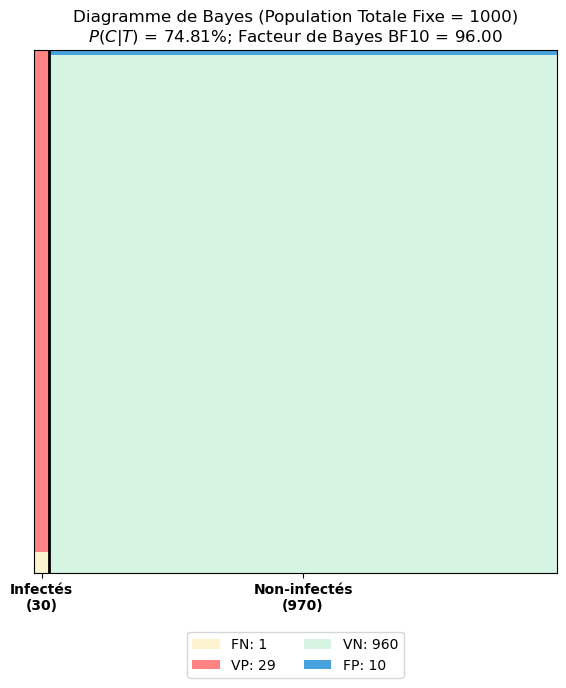
\includegraphics[width=0.5\linewidth]{Images/diagramme_bayes_crise}
		\label{fig:diagramme_bayes_crise}
	\end{figure}
\end{frame}

\begin{frame}{Période d'accalmie}
	En période d'accalmie, supposons que nous avons un test positif. Quelle est la probabilité d'avoir la Covid 19 avec un test positif ?
	\begin{itemize}
		\item La probabilité a priori d'avoir la Covid 19: $P(C) = 0.001$. 
		\item La sensibilité du test est de 96\% donc: $P(T \mid C) = 0.96$.
		\item La spécificité du test est de 99\% donc: $P(\bar{T} \mid \bar{C}) = 0.99$.
	\end{itemize}
	\vspace{0.5cm}
	\pause
	Faisons un raisonnement rapide pour un groupe de 1000 personnes:
	\begin{itemize}
		\item Il y a une personne infectée. On supposera que cette personne a un test positif.
		\pause
		\item Il y a 999 personnes non-infectées. Comme il y a 1\% d'avoir un faux positif, cela fait environ 10 personnes à avoir un faux positif.
		\pause
		\item Il y a donc 11 personnes avec un test positif. Et 10 d'entre elles ne sont pas infectées. Cela signifie donc qu'une personne avec un test positif a approximativement 9\% de chance d'être infectée.
	\end{itemize}
\end{frame}

\begin{frame}{Période d'accalmie - Calcul}
	La probabilité marginale est:
	\begin{equation}
		\begin{aligned}
			P(T) &= P(T \cap C) + P(T \cap \bar{C}) \\
			&= P(T \mid C) P(C) + P(T \mid \bar{C}) P(\bar{C}) \\
			&= P(T \mid C) P(C) + (1 - P(\bar{T} \mid \bar{C})) (1 - P(C)) \\
			&= 0.96 \times 0.001 + (1 - 0.99) \times (1 - 0.001) \\
			&= 0.00096 + 0.00999 = 0.01095
		\end{aligned}
		\nonumber
	\end{equation}
	\pause
	On peut donc calculer la probabilité a posteriori:
	\begin{equation}
		\begin{aligned}
			P(C \mid T) &= \frac{P(T \mid C) P(C)}{P(T)} \\
			&= \frac{0.96 \times 0.001}{0.01095} 
			= \frac{0.00096}{0.01095} \\
			&\approx 0.088
		\end{aligned}
		\nonumber
	\end{equation}
\end{frame}

\begin{frame}{Période d'accalmie - Visualisation}
	\begin{figure}
		\centering
		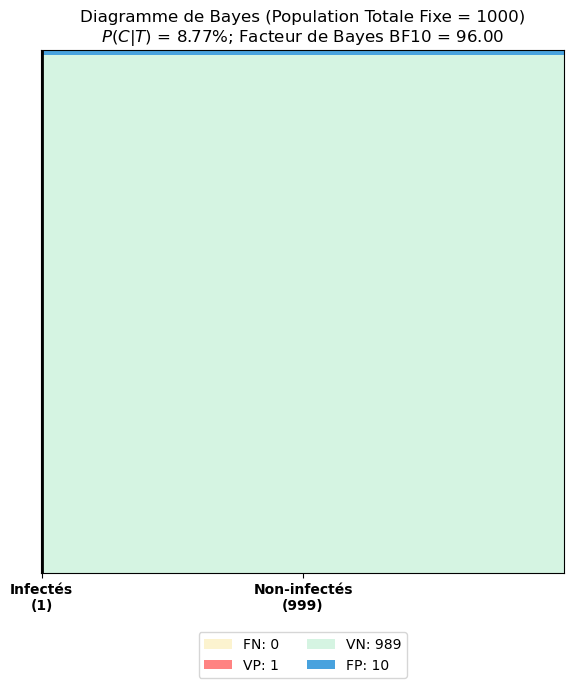
\includegraphics[width=0.5\linewidth]{Images/diagramme_bayes_accalmie}
		\label{fig:diagramme_bayes_accalmie}
	\end{figure}
\end{frame}


\begin{frame}{Période d'accalmie avec un second test positif}
	En période d'accalmie, supposons que nous avons un \textbf{second} test positif. On suppose ce test indépendant du premier. Quelle est la probabilité d'avoir la Covid 19 avec un second test positif ?
	\begin{itemize}
		\item La probabilité a priori d'avoir la Covid 19: $P(C) = 0.088$. C'est la probabilité d'avoir la Covid 19 après un premier test positif.
		\item La sensibilité du test est de 96\% donc: $P(T \mid C) = 0.96$.
		\item La spécificité du test est de 99\% donc: $P(\bar{T} \mid \bar{C}) = 0.99$.
	\end{itemize}
\end{frame}

\begin{frame}{Période d'accalmie avec un second test positif - Calcul}
	La probabilité marginale est:
	\begin{equation}
		\begin{aligned}
			P(T) &= P(T \cap C) + P(T \cap \bar{C}) \\
			&= P(T \mid C) P(C) + P(T \mid \bar{C}) P(\bar{C}) \\
			&= P(T \mid C) P(C) + (1 - P(\bar{T} \mid \bar{C})) (1 - P(C)) \\
			&= 0.96 \times 0.088 + (1 - 0.99) \times (1 - 0.088) \\
			&= 0.08448 + 0.00912 = 0.0936
		\end{aligned}
		\nonumber
	\end{equation}
	\pause
	On peut donc calculer la probabilité a posteriori:
	\begin{equation}
		\begin{aligned}
			P(C \mid T) &= \frac{P(T \mid C) P(C)}{P(T)} \\
			&= \frac{0.96 \times 0.088}{0.0936} 
			= \frac{0.08448}{0.0936} \\
			&\approx 0.903
		\end{aligned}
		\nonumber
	\end{equation}
\end{frame}

\subsection{Facteur de Bayes}

\begin{frame}{Introduction d'une forme alternative}
	Nous avons vu que le théorème de Bayes pour deux événements $A$ et $B$ s'écrit:
	\begin{equation}
		P(A \mid B) = \frac{P(B \mid A) P(A)}{P(B)}
		\nonumber
	\end{equation}
	\pause
	D'une manière similaire, on peut écrire:
	\begin{equation}
		P(\bar{A} \mid B) = \frac{P(B \mid \bar{A}) P(\bar{A})}{P(B)}
		\nonumber
	\end{equation}
	\pause
	En divisant ces deux relations:
	\begin{equation}
		\frac{P(A \mid B)}{P(\bar{A} \mid B)} = \frac{\frac{P(B \mid A) P(A)}{P(B)}}{\frac{P(B \mid \bar{A}) P(\bar{A})}{P(B)}}
		\nonumber
	\end{equation}	
\end{frame}

\begin{frame}{Facteur de Bayes}
	L'expression précédente se simplifie en:
	\begin{equation}
		\frac{P(A \mid B)}{P(\bar{A} \mid B)} = \frac{P(B \mid A)}{P(B \mid \bar{A})} \frac{P(A)}{P(\bar{A})}
		\nonumber
	\end{equation}
	\begin{block}{Définition: Facteur de Bayes}
		Soient deux événements $A$ et $B$, le facteur de Bayes est défini par:
		\begin{equation}
			\begin{cases}
				\text{BF}_{10}(B) = \displaystyle \frac{P(B \mid A)}{P(B \mid \bar{A})} \\[10pt]
				\text{BF}_{10}(\bar{B}) = \displaystyle \frac{P(\bar{B} \mid A)}{P(\bar{B} \mid \bar{A})}
			\end{cases}
			\nonumber
		\end{equation}
	\end{block}
	Note: l'indice $10$ signifie que la condition $A$ est vraie dans le numérateur et qu'elle est fausse dans le dénominateur. On aurait pu tout aussi bien définir un facteur de Bayes $\text{BF}_{01}$.
\end{frame}

\begin{frame}{Forme alternative du théorème de Bayes}
	En utilisant le facteur de Bayes, nous avons une forme alternative du théorème de Bayes utilisant les cotes:
	\begin{equation}
		\cote(A \mid B) = \text{BF}_{10}(B) \, \cote(A)
		\nonumber
	\end{equation}
	\pause
	Nous pouvons appliquer cette formulation pour notre problème de la Covid 19. Comme la sensibilité est de 96\% et la spécificité est de 99\%, on peut calculer le facteur de Bayes:
	\begin{equation}
		\begin{aligned}
			\text{BF}_{10}(T) &= \frac{P(T \mid C)}{P(T \mid \bar{C})} \\
			&= \frac{P(T \mid C)}{1 - P(\bar{T} \mid \bar{C})} \\
			&= \frac{0.96}{1 - 0.99} \\
			&= 96
		\end{aligned}
		\nonumber
	\end{equation}
\end{frame}

\begin{frame}{Forme alternative du théorème de Bayes}
	Nous pouvons utiliser ce facteur de Bayes pour résoudre les problèmes précédents. Il nous suffit de calculer la cote associée à la probabilité a priori. On rappelle que:
	\begin{equation}
		\cote = \frac{p}{1 - p}  \Longleftrightarrow p = \frac{\cote}{\cote + 1}
		\nonumber
	\end{equation}
	\begin{itemize}
		\item Si la probabilité a priori est de 3\%, la cote est $3:97$, et donc la cote a posteriori est $288:97$. Ce qui donne une probabilité a posteriori de 0.748.
		\item Si la probabilité a priori est de 0.1\%, la cote est $1:999$, et donc la cote a posteriori est $96:999$. Ce qui donne une probabilité a posteriori de 0.088.
		\item Si la probabilité a priori est de 8.8\%, la cote est $11:114$, et donc la cote a posteriori est $1056:114$. Ce qui donne une probabilité a posteriori de 0.903.
	\end{itemize}
\end{frame}

\subsection{Nature récursive du théorème de Bayes}

\begin{frame}{Critiques de cinéma}
	Un nouveau film vient de sortir au cinéma. On représentera notre avis par une variable aléatoire $A$ qui vaut 0 si on a un avis négatif sur le film et 1 sinon. Comme nous n'avons aucun avis précis sur le film, nous représenterons notre avis \textbf{a priori} par la fonction de masse suivante:
	\begin{equation}
		\begin{cases}
			P(A = 0) = 0.5 \\
			P(A = 1) = 0.5
		\end{cases}
		\nonumber
	\end{equation}
	\pause
	Nous lisons ensuite une série de critiques $C$, que l'on suppose indépendantes, qui peuvent être soit négatives $C=0$, soit positives $C=1$. Il nous faut aussi définir une sensibilité et une spécificité:
	\begin{itemize}
		\item \textbf{Sensibilité}: probabilité que la critique soit positive pour un film sur lequel on aurait un avis positif: 0.65
		\item \textbf{Spécificité}: probabilité que la critique soit négative pour un film sur lequel on aurait un avis négatif: 0.75
	\end{itemize}
\end{frame}

\begin{frame}{Critiques de cinéma - Visualisation}
	\begin{columns}
		\begin{column}{0.45\textwidth}
			Après avoir lu 2 critiques négatives et 2 critiques positives, nous avons maintenant un avis légèrement favorable sur le film. Pour obtenir ce résultat nous avons appliqué le théorème de Bayes 4 fois consécutives en utilisant la probabilité a posteriori du calcul précédent comme la probabilité a priori du calcul courant:
		\end{column}
		\begin{column}{0.55\textwidth}
			\begin{figure}
				\centering
				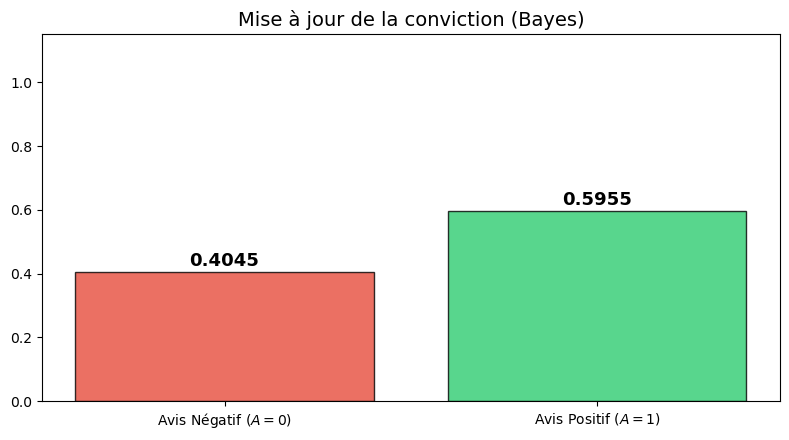
\includegraphics[width=1.0\linewidth]{Images/bayes_recursif}
				\label{fig:bayes_recursive}
			\end{figure}
		\end{column}		
	\end{columns}
	\vspace{0.5cm}
	Note: utiliser les facteurs de Bayes $\text{BF}_{10}(C=1)$ et $\text{BF}_{10}(C=0)$ rend le problème très rapide à résoudre:
	\begin{equation}
		\cote_{finale} = \text{BF}_{10}(C=0)^2 \text{BF}_{10}(C=1)^2 \cote_{initiale}
		\nonumber
	\end{equation}
\end{frame}

\subsection{Conclusion}

\begin{frame}{L'essentiel du raisonnement bayésien}
	L'inférence bayésienne n'est pas qu'une formule, c'est une \textbf{méthode de mise à jour des connaissances}.
	\vspace{0.3cm}
	\begin{itemize}
		\item \textbf{Le poids du contexte} : La probabilité \textit{a posteriori} dépend autant de la qualité de la preuve (vraisemblance) que de ce que l'on savait avant (a priori). 
		\begin{itemize}
			\item[$\rightarrow$] \textit{Un test excellent sur une maladie rare produit surtout des faux positifs.}
		\end{itemize}
		\pause
		\item \textbf{Le Facteur de Bayes ($BF_{10}$)} : C'est le multiplicateur de conviction. Il mesure la force intrinsèque d'une donnée, indépendamment du contexte.
		\pause
		\item \textbf{La nature récursive} : L'\textit{a posteriori} d'aujourd'hui est l'\textit{a priori} de demain. C'est le principe de l'apprentissage continu.
	\end{itemize}
\end{frame}

